\clearpage
\section{LW1 — Cinemática direta}
\textbf{Fontes:} \source{lw1\_medicoes.csv}, \source{lw1\_fk\_sim.csv}, \source{lw1\_fk\_real.csv}, esboço fornecido pelo grupo e folha de parâmetros UFACTORY. A implementação avaliada está em \source{src/lite6\_kinematics/lite6\_kinematics/forward\_kinematics.py}.

\subsection{Parte A — Referenciais e medição}
O referencial de base é \source{link\_base} e o terminal é \source{link\_eef}. A figura é o esboço original na configuração de juntas zero; foi fornecido com 267$\times$452 píxeis, pelo que a tabela numérica a seguir fixa os parâmetros. A implementação usa a convenção \textbf{DH standard}, conforme indicado pelo docente; a tabela e a ordem das transformações abaixo seguem essa convenção, embora os nomes das funções do template mantenham \source{dh\_table} e \source{mdh\_transform}.

\begin{center}
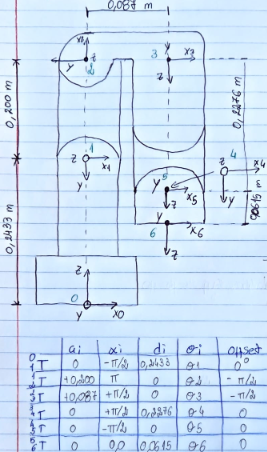
\includegraphics[height=0.31\textheight,keepaspectratio]{images/lw1_esboco.png}
\captionof{figure}{Esboço original das juntas, eixos, comprimentos e desvios angulares (LW1 A.1).}
\end{center}

A medição foi feita lendo apenas as juntas e a pose terminal em sete configurações: zero e uma rotação de cerca de $90^\circ$ por junta. O ficheiro guarda também quaternião, eixo $z$ terminal e código de erro (zero em todas as linhas). Não se usou URDF ou o modelo do Gazebo para extrair parâmetros.
\begin{center}\small
\begin{tabular}{@{}lrrrr@{}}\toprule
Configuração & $q$ variado & $x$ (mm) & $y$ (mm) & $z$ (mm)\\\midrule
zero & — & 87,00 & 0,00 & 153,59\\
J1 $+90^\circ$ & J1 & 0,00 & 87,00 & 153,59\\
J2 $+90^\circ$ & J2 & -89,91 & 0,00 & 156,50\\
J3 $+90^\circ$ & J3 & 290,12 & 0,00 & 530,69\\
J4 $+90^\circ$ & J4 & 86,99 & 0,00 & 153,59\\
J5 $+90^\circ$ & J5 & 24,50 & 0,00 & 216,09\\
J6 $+90^\circ$ & J6 & 87,00 & 0,00 & 153,59\\\bottomrule
\end{tabular}
\captionof{table}{Medições usadas na identificação geométrica.}
\end{center}
O ensaio de J1 confirma a rotação da projeção horizontal $(87,0)\to(0,87)$ mm. J4 e J6, na pose zero, mudam principalmente a orientação; J5 desloca a ponta de $(87,153{,}59)$ para $(24{,}5,216{,}09)$ mm no plano $xz$, dando escala de cerca de 62,5 mm para o avanço terminal. Os ensaios orientam a atribuição dos eixos e offsets; não identificam isoladamente todos os comprimentos com precisão submilimétrica. Para os valores nominais finais usou-se a tabela standard da folha do fabricante, comparada com estas observações.

\subsection{Tabela DH, comparação e implementação}
Na convenção standard, cada transformação é
\begin{equation}
{}^{i-1}T_i=R_z(q_i+\theta_{0,i})\,T_z(d_i)\,T_x(a_i)\,R_x(\alpha_i),
\qquad {}^0T_6=\prod_{i=1}^{6}{}^{i-1}T_i .
\end{equation}
\begin{center}\small
\begin{tabular}{@{}crrrr@{}}\toprule
$i$ & $a_i$ (m) & $\alpha_i$ & $d_i$ (m) & $\theta_{0,i}$\\\midrule
1 & 0 & $-\pi/2$ & 0,2433 & 0\\
2 & 0,2000 & $\pi$ & 0 & $-\pi/2$\\
3 & 0,0870 & $\pi/2$ & 0 & $-\pi/2$\\
4 & 0 & $\pi/2$ & 0,2276 & 0\\
5 & 0 & $-\pi/2$ & 0 & 0\\
6 & 0 & 0 & 0,0615 & 0\\\bottomrule
\end{tabular}
\captionof{table}{Tabela efetivamente implementada, com $\theta_i=q_i+\theta_{0,i}$ em radianos.}
\end{center}
Esta tabela coincide linha a linha com \emph{Standard D-H Parameters} da folha UFACTORY após converter mm para m e graus para radianos; a folha inclui também uma tabela \emph{Modified D-H Parameters}, com outra atribuição de referenciais e outra distribuição de $a$, $d$ e $\alpha$. Não se comparam linhas das duas convenções como se descrevessem o mesmo referencial intermédio. A pose terminal nominal em zero calculada por este modelo é $(87,0,154{,}20)$ mm; a medição e o TF do modelo são cerca de $(87,0,153{,}59)$ mm, diferença de cerca de $0{,}61$ mm em $z$. Esta discrepância entre parâmetros nominais e modelo de validação aparece nos erros medidos.

A função \source{dh\_table(q)} adiciona offsets ao vetor em radianos; \source{mdh\_transform()} constrói a matriz standard acima apesar do nome legado; \source{forward\_kinematics()} acumula as seis matrizes e, opcionalmente, devolve os sete referenciais. O nó \source{FkNode} lê juntas por nome de \source{/joint\_states} e publica a pose em \source{/lite6\_fk/pose}, copiando a marca temporal. Não se usou tf ou URDF no cálculo do grupo.

\subsection{Partes C e D — Verificação e validação}
Para uma pose calculada $(R_c,\mathbf p_c)$ e uma referência $(R_m,\mathbf p_m)$, foram usados os erros separados do enunciado:
\begin{equation}
e_p=\|\mathbf p_c-\mathbf p_m\|_2,\qquad
e_o=\arccos\!\left(\frac{\operatorname{tr}(R_c^\top R_m)-1}{2}\right).
\end{equation}
O \source{fk\_check} percorreu P0--P9 em Gazebo e depois no braço. A tabela mostra erros por configuração; os CSV incluem as juntas atingidas, matrizes e marcas temporais.
\begin{center}\scriptsize
\begin{tabular}{@{}lrrrrrr@{}}\toprule
& \multicolumn{2}{c}{Gazebo: vs. TF} & \multicolumn{2}{c}{Braço: vs. TF} & \multicolumn{2}{c}{Braço: vs. controlador}\\
Pose & mm & graus & mm & graus & mm & graus\\\midrule
P0 & 0,611 & 0,0008 & 0,611 & 0,0008 & 1,268 & 0,0078\\
P1 & 0,626 & 0,0012 & 0,626 & 0,0012 & 3,093 & 0,4697\\
P2 & 0,643 & 0,0013 & 0,643 & 0,0013 & 4,072 & 0,6291\\
P3 & 0,653 & 0,0011 & 0,653 & 0,0011 & 2,227 & 0,4154\\
P4 & 0,803 & 0,0014 & 0,803 & 0,0014 & 4,111 & 0,7393\\
P5 & 0,982 & 0,0010 & 0,982 & 0,0010 & 1,291 & 0,3851\\
P6 & 0,620 & 0,0009 & 0,620 & 0,0009 & 2,424 & 0,4135\\
P7 & 0,895 & 0,0014 & 0,895 & 0,0014 & 4,066 & 0,6837\\
P8 & 0,613 & 0,0010 & 0,613 & 0,0010 & 2,473 & 0,2132\\
P9 & 0,899 & 0,0010 & 0,897 & 0,0010 & 3,750 & 0,5318\\\midrule
Máximo & 0,982 & 0,0014 & 0,982 & 0,0014 & 4,111 & 0,7393\\\bottomrule
\end{tabular}
\captionof{table}{Erros por pose de \source{lw1\_fk\_sim.csv} e \source{lw1\_fk\_real.csv}; arredondamento apenas para apresentação.}
\end{center}
As dez posições foram registadas em cada ambiente, sem rejeição na execução real final. P1.3 (Gazebo vs. TF, $<2$ mm e $<0{,}05^\circ$) é cumprido, inclusive os alvos de $1{,}5$ mm e $0{,}01^\circ$. P1.4 exige comparação \emph{com o controlador real}, com limiar $<3$ mm e $<0{,}1^\circ$: o máximo medido de $4{,}111$ mm e $0{,}7393^\circ$ \textbf{não cumpre}. A concordância com TF não substitui essa referência. Os dados não permitem atribuir causa única à diferença; parâmetros/calibração do controlador, definição de TCP e instante de amostragem exigiriam investigação. P1.2 depende de referência e poses ocultas do docente; não é declarado aprovado com estes ficheiros.

\textbf{Vídeo.} \href{\repo/lw1/lw1_fk_real.mp4}{Execução da LW1 no braço}: o verificador pede confirmação antes de cada movimento e regista P0--P9. O ficheiro tem 90,24 s.
